\subsection{Initialisierung der Navigation}

\begin{figure}[H]
\centering
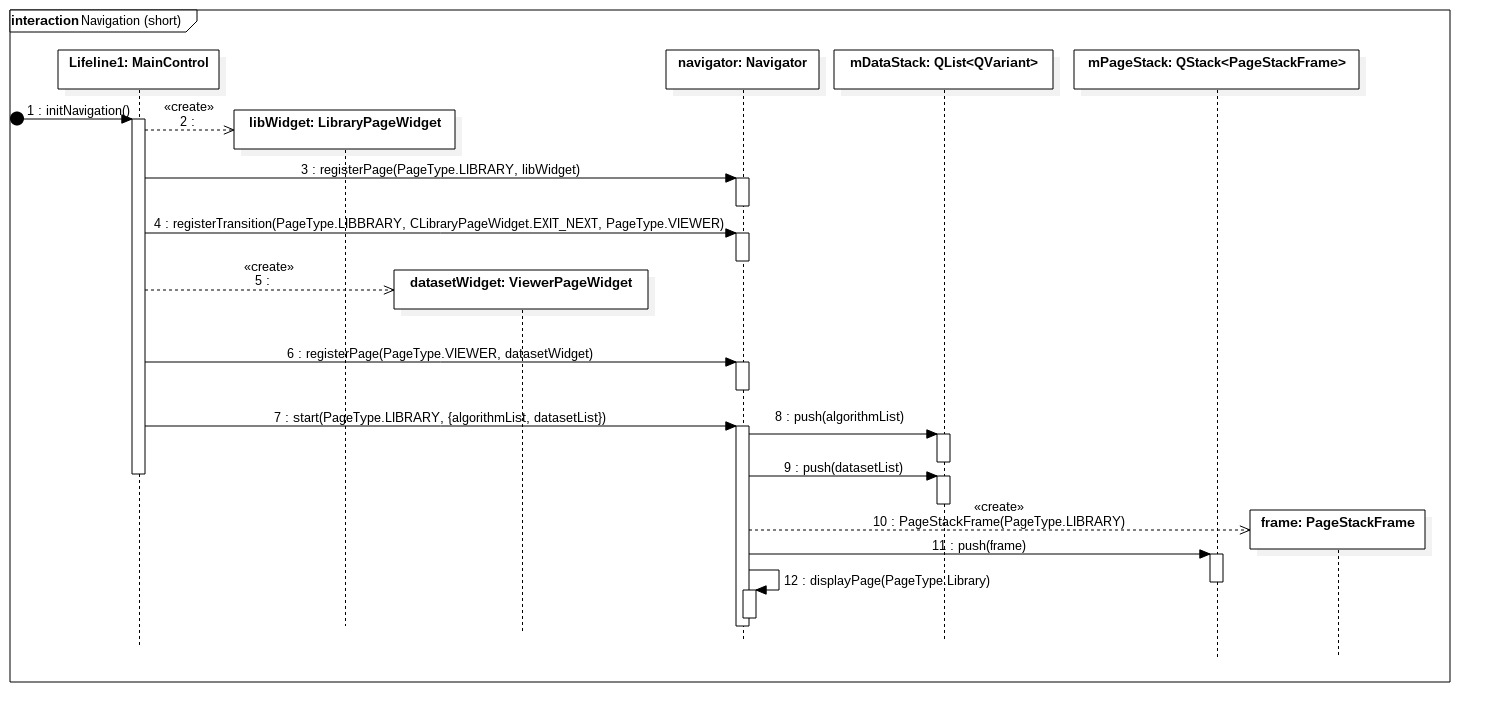
\includegraphics[width=\linewidth]{img/Sequenzdiagramme/Interaction}
\label{fig:Navigation init}
\end{figure}

Dieses Sequenzdiagramm beschreibt die Abläufe beim Programmstart, wenn MainControl die verschiedenen Komponente initilisiert.

\begin{itemize}
	\item initNavigation() wird aufgerufe

	\item MainControl erstellt LibraryPageWidget

	\item MainControl registriert LibraryPageWidget und Übergang zum ViewerPageWidget

	\item MainControl erstellt ViewerPageWidget und registriert beim Navigator

	\item Startet Navigator mit LibraryView

	\item Füge Suchdaten in DataStack ein

	\item Erstellt ein PageStackFrame für Library und füge dies in PageStack hinzu

	\item Zeige Library an.

\end{itemize}

\pagebreak

\subsection{Seitenwechsel}

\begin{figure}[H]
\centering
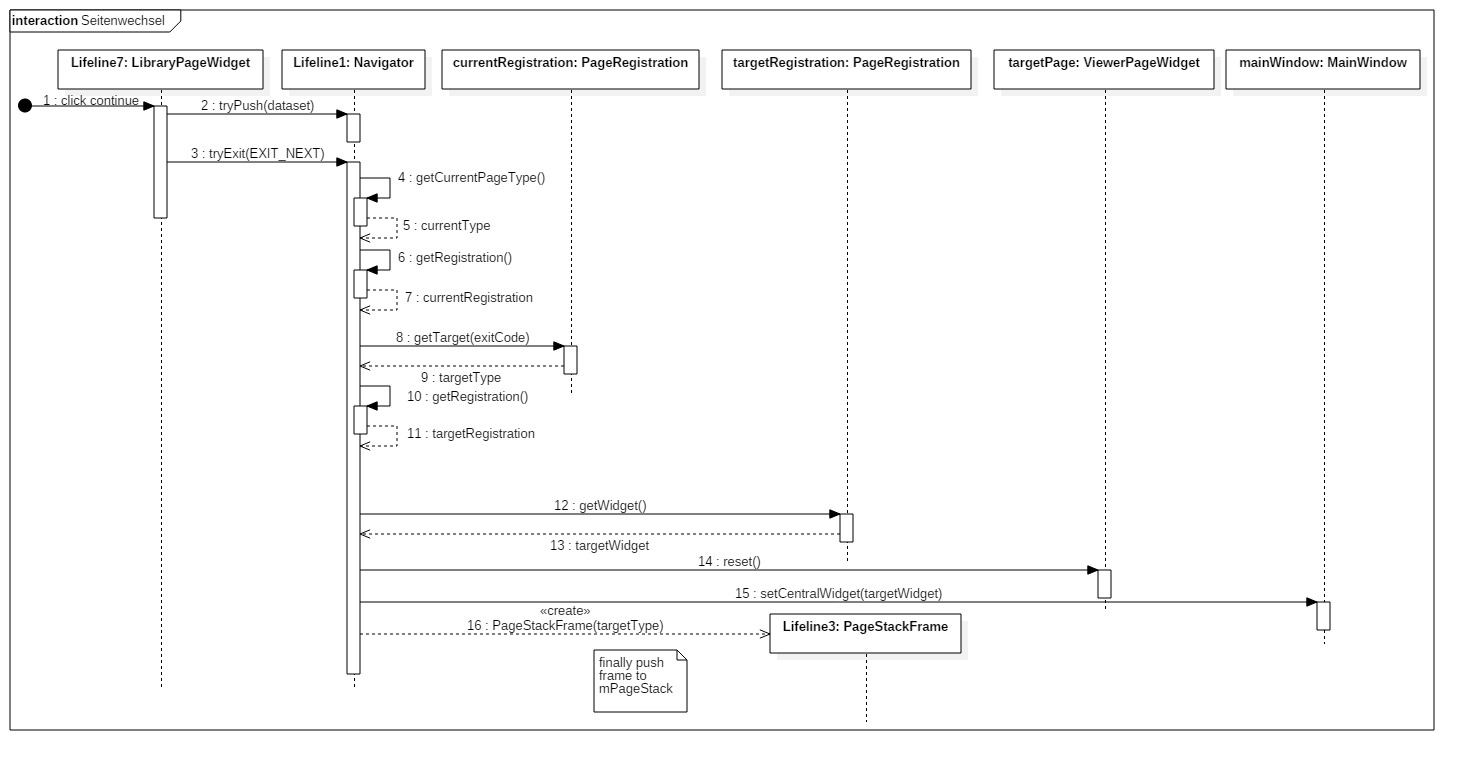
\includegraphics[width=\linewidth]{img/Sequenzdiagramme/Seitenwechsel}
\label{fig:seitenwechsel}
\end{figure}

Dieses Sequenzdiagramm beschreibt die Abläufe beim Seitenwechsel vom LibraryPageWidget zum ViewerPageWidget

\begin{itemize}
	\item Benutzer klickt auf 'weiter' (Library)

	\item Datensatz wird an Navigator gesendet

	\item LibraryPageWidget sendet Navigator einen Exit-Code, um die Seite zu wechseln

	\item Als PageType wird LIBRARY zurückgegeben. Die entsprechenede PageRegistration wird ermittelt, aus der PageType der nächster Seite lesen läss

	\item Aufruf der Funktion, ein PageWidget anhand PageType anzuzeigen

	\item ViewerPageWidget wird wiederum aus PageRegistration abgelesen.

	\item Der Navigator registriert das ViewerPageWidget als das PageWidget, das danach angezeigt werden soll. Das MainWindow erhält dies

\end{itemize}

\pagebreak

\subsection{Suche starten}

\begin{figure}[H]
\centering
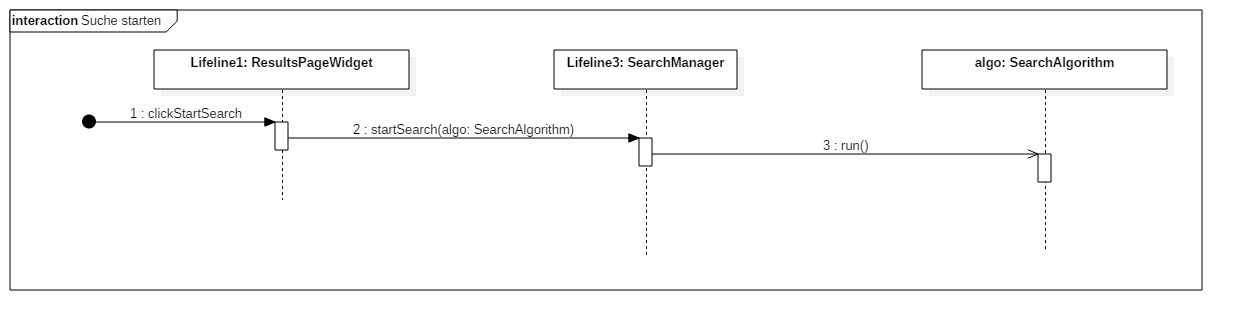
\includegraphics[width=\linewidth]{img/Sequenzdiagramme/SucheStarten}
\label{fig:sucheStarten}
\end{figure}
Nachdem der Benutzer den Button zum Start der Suche geklickt hat, übergibt das aktuelle PageWidget den Algorithmus an den SearchManager. Dieser startet die Suche.

\subsection{Suche terminieren}

\begin{figure}[H]
\centering
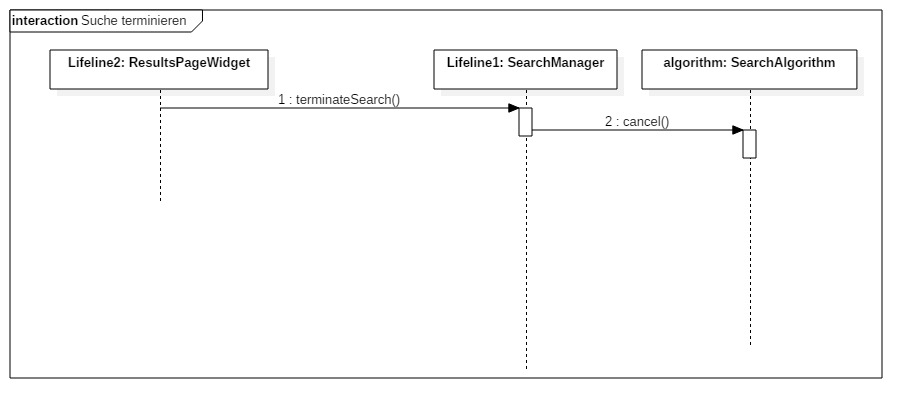
\includegraphics[width=\linewidth]{img/Sequenzdiagramme/SucheTerminieren}
\label{fig:sucheTerminieren}
\end{figure}
Das ResultsPageWidget veranlasst den SearchManager dazu, den Algorithmus zu beenden.

\subsection{Suchergebnis speichern}

\begin{figure}[H]
\centering
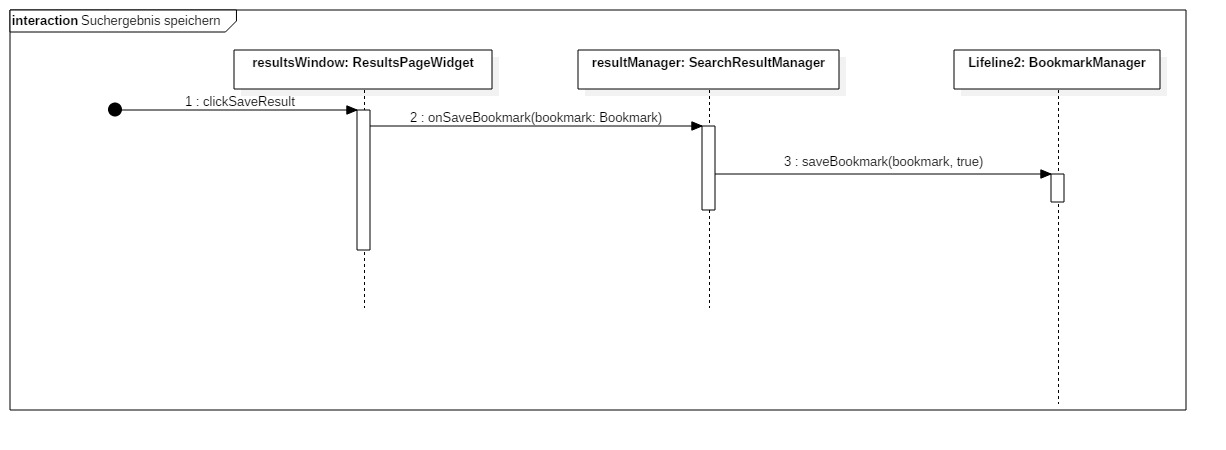
\includegraphics[width=\linewidth]{img/Sequenzdiagramme/SuchergebnisSpeichern}
\label{fig:suchergebnisSpeichern}
\end{figure}
Nachdem der Benutzer den Button zum Speichern des Suchergebnisses geklickt hat, übergibt das ResultsPageWidget dem SearchResultManager das Bookmark. Dieser ruft den BookmarkMangager zum Speichern auf.